
\documentclass[a4paper,11pt]{amsart}%

\usepackage{ifxetex}
\usepackage{ifpdf}
\usepackage{multicol}
\usepackage{bm}

\newcommand{\comment}[1]{}
\newcommand{\code}[1]{\texttt{#1}}
\newif\ifforauthor

%%%%%%%%%%%%% Packages %%%%%%%%%%%%%%%%%
\usepackage{amssymb, amsthm,amsmath}

\ifpdf
  \usepackage{graphicx}
  \usepackage{hyperref}
\else
  \ifxetex
    \usepackage{graphicx}
    \usepackage{hyperref}
  \else
    \usepackage[dvipdfm]{graphicx}
    \usepackage[dvipdfm]{hyperref}
  \fi
\fi
\graphicspath{{./img/}}

\usepackage{enumitem}
\usepackage{caption}
\usepackage{soul, color}
\newcommand\jc[1]{\hl{{\bf jc:} #1}}

\usepackage{listings}
\lstset{
  frame=single,
  breaklines=true,
  basicstyle=\fontsize{7}{13}\selectfont\ttfamily
}

\hypersetup{
bookmarksnumbered=true,
colorlinks=true,
pdfstartview={FitH},
linkcolor=blue
}

%%%%%%%%%%%%%%%%%%%%%%%%%%%%%%%%%%%%%%%
\newcommand\sep{\,:\,}
\newcommand{\vSpace}{\vspace{5mm}\noindent}
\newcommand{\vSmall}{\vspace{3mm}\noindent}
\newcommand\fakesection[1]{\noindent{\bf #1}\\}
\newcommand\bs{\backslash}
\newcommand\A{\mathbb{A}}
\newcommand\Z{\mathbb{Z}}
\newcommand\Q{\mathbb{Q}}
\ifxetex
  \renewcommand\C{\mathbb{C}} %renewcommand using xelatex
\else
  \newcommand\C{\mathbb{C}}
\fi
\newcommand\pgl{\operatorname{PGL}}
\newcommand{\eLL}{{\mathcal L}}
\newcommand\algno{\overline\Q}
\newcommand\R{\mathbb{R}}
\newcommand\adj{\operatorname{adj}}
\renewcommand\P{\mathbb{P}}
\newcommand{\N}{\mathbb{N}}
\newcommand\wo[1]{\backslash{\{#1\}}}
\newcommand\spn[1]{\langle #1 \rangle}
\newcommand\pmat[1]{\begin{pmatrix} #1 \end{pmatrix}}
\newcommand\authortext[1]{\ifforauthor {\color{red}#1} \fi}
%\renewcommand\st{\mathrel{\ooalign{$\,\backepsilon$\cr\lower .7pt\hbox{\kern 1pt$-\,$}}}}
%%%%%%%%%%%%%%% TITLE %%%%%%%%
%\title{Template for TeX files}
\title{}
\date{}
\thispagestyle{empty}
%%%%%%%%%%%%%%%%%%%%%%%%%%%
\theoremstyle{definition}
\newtheorem{theorem}{Theorem}[section]
\newtheorem*{defi}{Definition}
\newtheorem*{nota}{Notation}
\newtheorem{remark}[theorem]{Remark}
\newtheorem{lemma}[theorem]{Lemma}
\newtheorem{cor}[theorem]{Corollary}
\newtheorem{prop}[theorem]{Proposition}
\newtheorem{exam}[theorem]{Example}
\newtheorem{const}[theorem]{Construction}
%%% free theorem styles
\newcommand{\thistheoremname}{}
\newtheorem{genericthm}[theorem]{\thistheoremname}
\newenvironment{namedthm}[1]
  {\renewcommand{\thistheoremname}{#1}%
   \begin{genericthm}}
  {\end{genericthm}}
\newtheorem{none}[theorem]{}

\title{Exact Polynomial Sum of Squares Decompositions}

\author{Jose Capco}
\address{Universit\"at Innsbruck - Austria}
\email{jose.capco@uibk.ac.at}
\author{Santiago Laplagne}
\address{Departamento de Matem\'atica, FCEN, Universidad de Buenos Aires - Ciudad Universitaria,
Pabell\'on I - (C1428EGA) - Buenos Aires, Argentina}
%\curraddr{}
\email{slaplagn@dm.uba.ar}
\author{Claus Scheiderer}
\address{Universit\"at Konstanz - Germany}
\email{claus.scheiderer@uni-konstanz.de}

\begin{document}

\begin{abstract}
We construct two examples of non-negative polynomials over $\Q$ that can be decomposed as sum of squares over $\Q(\alpha)$, for $\alpha$ the real root of $X^3-2$, but not over $\Q$. The first example is a polynomial in $3$ variables of degree $6$ and the second example is a polynomial of degree $4$ in $4$ variables. Furthermore, we show how to modify the construction to construct families of examples over more general algebraic extensions of degree 3.
\end{abstract}
\maketitle

\section{Introduction}
Determining if a given polynomial can be expressed as sums of squares of polynomials (SOS), and compute such decompositions, is a fundamental problem in real algebraic geometry. We address the problem of determining when a rational polynomial that can be decomposed as a sum of squares of real polynomials ($\R$-SOS) can also be decomposed as a sum of squares over the rational numbers ($\Q$-SOS).

In \cite{scheiderer} the first families of negative examples were found (that is, rational polynomials that are $\R$-SOS but not $\Q$-SOS). Moreover, for the case of polynomials of degree 4 in 3 variables (shortly, the (3,4) case), the author gives a complete characterization of the negative examples. In particular, all such examples are sum of two squares with coefficients in algebraic extensions of $\Q$ of even degree.

In \cite{laplagne} a new negative example was found, given by a polynomial of degree 6 in 4 variables, with coefficients over an algebraic extension of $\Q$ of odd degree 3. The verification uses computational techniques difficult to extend to families of polynomials. It remained as an interesting question to study the smaller cases of polynomials of degree 6 in 3 variables and degree 4 in 4 variables (that is, the (3,6) and (4,4) cases). The general study of the SOS cone in these two cases has attracted a lot of interest recently (see \cite{blekherman}, \cite{blekherman2}, \cite{capco}).

In our work, following the construction in \cite{laplagne}, we provide new examples of non-negative polynomials that are $\R$-SOS but not $\Q$-SOS for both of those cases. Most interestingly, we are able to provide more general theoretical proofs that these polynomials cannot be decomposed as $\Q$-SOS, and that the given decomposition is unique, which allows us to extend the results to new families of counterexamples, perturbing the coefficients and using more general degree 3 algebraic extensions.

\subsection{Basic construction}

Let $H_{n,d}$ be the vector space of homogeneous polynomials in $n$ variables of degree $d$ with coefficients in $\R$.

We recall from \cite{laplagne} the basic construction for polynomials over $\Q$ that are sum of
squares of polynomials in an algebraic extension of $\Q$. We restrict first to the case of sum of 3 polynomials over $\Q(\alpha)$, where $\alpha$ is the real cubic root of $2$.

\begin{namedthm}{SOS Construction}\label{ls_3sos}
Let $\bm x = x_0,\dots,x_n$. Let $\alpha$ be the real cubic root of $2$ and let
\begin{align*}
p_1 &= b_1b_2^2+b_1^3+b_1b_3^2-2a_3b_3c_1-2c_1c_2^2-2c_1^3
  +2a_3b_1c_3-2c_1c_3^2-2b_1b_2c_2\alpha,\\
  &+2b_2^2c_1\alpha-2b_1c_2^2\alpha^2+2b_2c_1c_2\alpha^2\\
p_2 &= b_1^2b_2+b_2^3+b_2b_3^2-2a_3b_3c_2-2c_1^2c_2-2c_2^3
  +2a_3b_2c_3-2c_2c_3^2-2b_1b_2c_1\alpha,\\
  &+2b_1^2c_2\alpha-2b_2c_1^2\alpha^2+2b_1c_1c_2\alpha^2\\
p_3 &= 2(b_2c_1-c_2b_1)(a_3+b_3\alpha+\alpha^2c_3),
\end{align*}
where $a_3,b_1,b_2,b_3,c_1,c_2,c_3$ are any choice of polynomials in $\Q[\bm x]$ such that $p_1,p_2,p_3$ are not
identically $0$. Then
$$p_1^2 + p_2^2 + p_3^2 \in \Q[\bm x].$$

One can verify the above by
checking that the coefficients of $\alpha$ and $\alpha^2$ vanish after computing the sum of squares. Notice also that
$p_2$ is just $p_1$ where $c_1$ is swapped with $c_2$ and $b_1$ is swapped with $b_2$.
\end{namedthm}

\begin{remark}
In the above construction, for simplicity, we only consider $b_1$, $b_2$, $b_3$, $c_1$, $c_2$, $c_3$, $a_3$ chosen as linear forms (or $0$) in $\Q[\bm x]$. The sum of squares in this case is a sextic form. However, we will see in the example with quaternary forms that we can choose them so that they have a common factor which can be mod out to obtain examples of smaller degree.
\end{remark}

\section{Polynomials in 3 variables of degree 6}
We construct an example of a polynomial of degree 6 in 3 variables that can be decomposed as a sum of squares over $\R$ but not over $\Q$.  In \cite{scheiderer}, C. Scheiderer studies the case of polynomials of degree 4 in 3 variables and gives a complete characterization of the
negative examples. In particular, all such examples are sum of two squares
with coefficients in an algebraic extensions of $\Q$ of even degree. In his proof, he uses strongly the fact that non-negative polynomials of degree 4 in 3 variables are always sum of squares.
The next example shows that the characterization provided in that paper cannot be extended to polynomials of degree 6. The example is constructed applying the following substitutions in Construction \ref{ls_3sos}:
\begin{align*}
  a_3 = z-x, && b_1 = x, && b_2 = y, && b_3 = y+z, && c_1 = z, && c_2 = z, && c_3 = x.
\end{align*}

\begin{prop}\label{3-6_nonQ} %\emph{$(3,6)$ Example with Unique Gram Matrix.}\\
For $\alpha$ the real root of $X^3-2$, define
{\footnotesize \begin{align*}
p_1 &=-2\alpha^2xz^2+2\alpha^2yz^2-2\alpha x^2z+2\alpha xyz+x^2y+2x^2z-4xyz-2xz^2-2y^3\\
&-2y^2z+yz^2+6z^3, \\
p_2 &= -2\alpha^2xz^2+2\alpha^2yz^2-2\alpha xyz+2\alpha y^2z-x^3+2xy^2+4xyz+3xz^2-2yz^2-6z^3,\\
p_3 &= 2z(x-y)((z-x) + \alpha (y+z) + \alpha^2 x),
\end{align*}}%
polynomials in $\Q(\alpha)_3[x, y, z]$ and let $f = p_1^2 + p_2^2 + p_3^2 \in \Q_6[x,y,z]$,
\begin{align*}
f&=x^6-3x^4y^2-4x^4yz+2x^4z^2-8x^3y^2z-8x^3yz^2+28x^3z^3+4x^2y^3z\\
&\quad+10x^2y^2z^2+24x^2yz^3+41x^2z^4+16xy^4z+32xy^3z^2-48xy^2z^3\\
&\quad-120xyz^4-60xz^5+4y^6+8y^5z-12y^3z^3-15y^2z^4+36yz^5+72z^6.
\end{align*}
Then $f$ is a sum of squares over $\Q(\alpha)$ but not over $\Q$.
\end{prop}



\begin{proof} See \cite{worksheets3644} for the computations in \code{Maple} \jc{the link is dead or perhaps wrong}. 
Let $K$ be the Galois closure of $\Q(\alpha)$. Then the common (projective) zeros of these four polynomials are all real points in $\P^3(K)$
and are given by:
\begin{multicols}{2}\noindent
\begin{align*}
P_1 &=(1:1:1),\\
P_2 &= (-2:-2:1),\\
P_3 &= (-3:-3:1),
\end{align*}
\begin{align*}
P_4 &= (1: \sqrt 2/2: 0),\\
P_5 &= (1: -\sqrt 2/2: 0).
\end{align*}
\end{multicols}

To show that the polynomial $f$ does not allow a $\Q$-SOS decomposition we can proceed as in \cite{laplagne}. We let $v$ be the set of all 10 monomials of degree 3 in 3 variables and consider the set of symmetric matrices $$\eLL := \{Q \in \R^{10 \times 10} | f(\bm x) = v(\bm x)^t Q v(\bm x)\}.$$

Using the 5 real roots of $f$ for facial reduction, we reduce to a $5 \times 5$ matrix in 2 variables:
\[
A = \frac{1}{2}
 \begin{pmatrix}
  2 & -4 + x & 0 & -x  & -2 + y \\
  -4 + x & 20 + 2y & 0 & -12-2y & 16 \\
  0 & 0 & 4 & x & 8 + y \\
  -x & -12 - 2y & 2x & -14 - y + 4x & 12 + x/2 \\
  -2 + y & 16 & 16 + 2y & 24 + x & 130 - 12x
 \end{pmatrix}.
\]

We need to find $x, y$ such that $A$ is positive semidefinite. This problem is harder to solve than what it might look like at first sight.
We were able to solve it using \texttt{RegularChains} \cite{RegularChains} package in \code{Maple} or \code{Cylindrical Algebraic Decomposition} \cite{CylindricalDecomposition} package in  \code{Mathematica}. In both cases the system is solved completely and we get that there is a unique solution which coincides with the one given by the original decomposition. So we conclude that the Gram spectrahedron consists of only one point with non-rational entries and hence there is no $\Q$-SOS decomposition for $f$.

\end{proof}

We now give an alternate proof that this polynomial cannot be expressed as the sum of polynomials over $\Q$. This proof is less computational, it only requires some basic linear algebra computations, and it can be more easily generalized to further examples.

\begin{proof}[\protect{Alternative proof of Proposition~\ref{3-6_nonQ}}]
\jc{are the computations for this alternative proof also in some Maple worksheet?}
Let $Z = \{P_1 =(1:1:1), P_2 = (-2:-2:1), P_3 = (-3:-3:1), P_4 = (1: \sqrt 2 / 2: 0), P_5 = (1: -\sqrt 2 / 2: 0)\}$ be the five common real zeros of $p_1$, $p_2$ and $p_3$. Let $W \subset H_{3,3}$ be the linear subspace consisting of all the cubic forms vanishing in $Z$. By an easy linear algebra computation we obtain a basis for $W$,
\begin{align*}
\mathcal{B}  =  & \{w_1 = p_1, w_2 = p_2, w_3 = p_3, w_4=x^2y-2y^3-4y^2z-yz^2+6z^3,  \\
& w_5=x^3-2xy^2-4y^2z-yz^2+6z^3\}
\end{align*}
%$w_1=x^2*z-x*y*z, w_2=x*y*z-y^2*z, w_3=x*z^2-y*z^2, w_4=x^2*y-2*y^3-4*y^2*z-y*z^2+6*z^3, w_5=x^3-x^2*y-2*x*y^2+2*y^3$
(note that since $H_{3,3}$ has dimension 10 and we have 5 conditions, the expected dimension for $W$ is indeed 5).

Let $W^2 \subset H_{3,6}$ be the set of all products $\{pq: p, q \in W\}$. It is generated by the 15 products $\{w_i w_j$, $1 \le i \le j \le 5\}$, and computing syzygies among these polynomials, we find two linear relations. Hence $\dim(W^2)=13$. We now wish to construct a linear form $\varphi: W^2 \rightarrow \R$ such that the associated bilinear form $\mathfrak{b}: W \times W \rightarrow \R$, $\mathfrak{b}(p,q) := \varphi(pq)$, has the following two properties:
\begin{enumerate}
\item $\mathfrak{b}$ is positive semidefinite,
\item the kernel of $\mathfrak{b}$ is equal to $U = \langle p_1, p_2, p_3 \rangle$.
\end{enumerate}

In the base $\mathcal{B}$ the matrix for $\mathfrak{b}$ must have the form
\[A =
\left(\begin{array}{c c c |c c}
	0 & 0 & 0 & 0 & 0 \\
	0 & 0 & 0 & 0 & 0 \\
	0 & 0 & 0 & 0 & 0 \\
	\hline
	0 & 0 & 0 & a & b \\
	0 & 0 & 0 & b & c \\
\end{array}\right)
\]
where the values of $a, b, c$ have to be chosen to satisfy the linear relations between the products $w_i w_j$, $1 \le i \le j \le 5$ in $W^2$. Plugging in those relations, we get a unique solution in up to linear scaling.
% Wrong relations
%\[
% b = a \left(-\frac{963}{1276} \alpha^2+\frac{48}{319} \alpha - \frac{723}{638}\right), c = a \left(\frac{15}{58}  \alpha^2+\frac{2347}{638}  \alpha + \frac{731}{638} \right),
%\]

Setting $a = 1$ we get the matrix
\[
\left(\begin{array}{c c}
	a & b \\
	b & c \\
\end{array}\right) \approx
\left(\begin{array}{c c}
	1 & -1. 1417 \\
	-1.1417 & 2.9078 \\
\end{array}\right),
\]
which is a positive definite matrix, and hence the resulting matrix $A$ is positive semidefinite.

To conclude the proof, assume now that we have a SOS representation $f = q_1^2 + \dots + q_r^2$. Clearly $q_i \in W$, $1 \le i \le r$, but then $0 = \mathfrak{b}(p_1^2) + \mathfrak{b}(p_2^2) + \mathfrak{b}(p_3^2) = \mathfrak{b}(f) =  \mathfrak{b}(q_1^2) + \dots + \mathfrak{b}(q_r^2)$. So $q_i \in \ker(\mathfrak{b}) = U$. That is, every polynomial in a SOS decomposition of $f$ is a linear combination of $p_1, p_2, p_3$.

It remains to show that there is no non-trivial linear combination of $p_1$, $p_2$ and $p_3$ with coefficients in $\Q$. Indeed, we consider a generic linear combination of $p_1$, $p_2$ and $p_3$, $g(c_1, c_2, c_3) = w_1 p_1 + w_2 p_2 + w_3 p_3$ and assume $g(c_1, c_2, c_3) \in \Q[x,y,z]$. The coefficient of $x_0^3$ is $w_2$, hence $w_2 \in \Q$ and the coefficient of $x_1^3$ is $w_1$, hence $w_1 \in \Q$. The coefficient of $y^2z$ is $-2\alpha w_2-2\alpha w_3+2w_1$, hence $w_3 = -w_2$. Now the coefficient of $x^2 z$ is $(2\alpha-2)w_1-2(\alpha^2-1)w_2$ and this implies $w_1 = 0$ and $w_2 = 0$.
\jc{here you are using $w_i$ are rational numbers, while you already reserved $w_i$ as elements in the basis $\mathfrak{B}$}
\end{proof}

\jc{I did not verify the paragraph below. We should share a script/worksheet that shows all this.}
As we mentioned before, we can easily get other examples in the neighborhood of $f$ by small perturbations of the coefficients of the construction.
We analyze an example perturbing the coefficient of $z$ in the expression of $b_3$. Let $b_3 = x + tz$ and all other variables as before.
The construction \ref{ls_3sos} yields a polynomial $f$ with 5 real roots:
\[
P_1, P_2 = (\alpha : \alpha : 1), P_3 = (-(t+2) : -(t+2) : 1), P_4, P_5 = (1 : \beta : 0),
\]
where $\alpha$ is a root of $X^2+tX-2$ (note that this give two real roots for any $t \in \R$) and $\beta$ is a root of $2X^2-1$.
Repeating the above construction we obtain a positive definite matrix for any $t$ in the interval $t \in T = (0.364425, 4.97349)$. That is, for any $t \in \Q \cap T$, we get a polynomial $f \in \Q[x,y,z]$ that can be decomposed as a sum of squares over $\R$ but not over $\Q$.

\section{Quaternary Forms}

We now consider the case of polynomials of degree 4 in 4 variables. We construct an example of a rational polynomial that is a sum of squares over $\R$ but not over $\Q$. In this case, the Gram spectrahedron does not consist of a single point. 

\begin{prop}\label{4-4}
For $\alpha$ the real root of $X^3-2$, define
\begin{align*}
p_1 &= -4\alpha^2x^2+4\alpha x^2-2x^2+y^2-2yz+2zw-2w^2, \\
p_2 &= -4\alpha^2x^2-4\alpha x^2+6x^2+y^2+2yz+2zw+2w^2, \\
p_3 &= 4x(\alpha^2w+\alpha y+z),
\end{align*}
polynomials in $\Q(\alpha)_2[x,y,z,w]$ and let $f=p_1^2+p_2^2+p_3^2\in \Q_4[x,y,z,w]$,
\begin{align*}
f&=40x^4+8x^2y^2+32x^2yz+64x^2yw+16x^2z^2+16x^2zw+\\
&+32x^2w^2+2y^4+8y^2z^2+8y^2zw+16yzw^2+8z^2w^2+8w^4.
\end{align*}

Then $f$ cannot be decomposed as a sum of squares of polynomials in $\Q$.
\end{prop}

\begin{proof} See \cite{worksheets3644} for the computations in \code{Maple}.
We have the following real vanishing points of $f$ in $\P^3$ \jc{this is written in $(x:y:z:w)$ order. Should we change it to $(w:x:y:z)$?}:
\begin{multicols}{2}\noindent
\begin{align*}
P_1&=(0:0:1:0),\\
P_2&=(0:2\alpha:-\alpha^2:2),
\end{align*}
\begin{align*}
P_3&=(\gamma:\beta:-\alpha-\alpha^2\beta:1),\\
P_4&=(-\gamma:\beta:-\alpha-\alpha^2\beta:1),
\end{align*}
\end{multicols}
\noindent where $\beta$ is the positive real root of $X^2+(\alpha^2-2\alpha)X-1$ and $\gamma,-\gamma$ are the two (real)
roots of $2X^2+2\alpha\beta+1$.

If we perform facial reduction using these four points, we reduce to a $10 \times 10$ matrix $Q$ of rank 6 in two unknowns $a, b$.
In this case the Gram matrix is not unique, but it is still easy to see that there is no rational matrix by inspecting the entries. 
We observe \jc{I did not compute the remaining observations. Do you have this in the worksheet?}
\begin{align*}
Q_{1,9} &= 8-(1/2) \alpha^2 a, \\
Q_{1,8} &= -(1/2) a,
\end{align*}
hence if $Q$ is rational it must be $a = 0$.
Substituting $a = 0$ in $Q$, we now observe that 
$$Q_{1,5} = (27/4) \delta^{10}+27 \delta^8+9\delta^6-88\delta^4-24\delta^2+48,$$
where $\delta$ is a root of $27 X^{12}+108X^{10}+36X^8-352X^6-48X^4+192X^2-64$. This polynomial is irreducible over $\Q$, hence $\Q(\delta)$ is an extension of degree 12 and therefore $Q_{1,5}$ is non--rational.
\end{proof}

\begin{remark}\label{remark:subs44}
The example was built using the following substitutions on Construction \ref{ls_3sos}:
\begin{align*}
  b_1 = x && b_2 = -x && b_3 = y && c_1 = -x && c_2 = -x && c_3 = w && a_3 = z.
\end{align*}
The resulting polynomials $p_1, p_2, p_3$ have $\alpha^2 w+\alpha y+z$ as common factor, and we divided out this factor to obtain polynomials of degree $2$.
\end{remark}

As for the case of ternary sextics, we provide an alternate more geometrical proof that this polynomial cannot be decomposed as a sum of squares in $\Q$.

\begin{proof}[\protect{Alternative proof of Proposition~\ref{4-4}}]
Let $p_1, p_2, p_3$ be as above. The polynomial $p_3$ splits as a product $p_3 = x \cdot l$ of two linear forms,
where $l = z + \alpha y + \alpha^2 w$.

The set $Z$ of common real zeros of $p_1$, $p_2$, $p_3$ therefore consists of
\begin{enumerate}
\item \label{branch1} the common real zeros $Z_1$ of $p_1$, $p_2$ in the plane $x = 0$;
\item \label{branch2} the common real zeros $Z_2$ of $p_1$, $p_2$ in the plane $l = 0$.
\end{enumerate}

In either case, we intersect two plane conics, so we expect 4 complex zeros each. In
either case, precisely two of the four are real, namely
\begin{itemize}
% {x = 0, y = 0, z = z, w = 0}
% {x = 0, y = RootOf(_Z^3-2)*w, z = -(1/2)*RootOf(_Z^3-2)^2*w, w = w}
\item in case (\ref{branch1}), $Z_1$ consists of the two points $P_1 = (0 : 0 : 1 : 0)$ and $P_2 = (0 : 2\alpha : -\alpha^2: 2)$ ($P_2$ two non--real conjugates);
\item in case (\ref{branch2}), the four complex points are Galois conjugate to each other over
$\Q(\alpha)$, and exactly two of them are real, i.e. in $Z_2$. They have coordinates
\[
P_3 =(\gamma:\beta:-\alpha-\alpha^2\beta:1), \ \
P_4 =(-\gamma:\beta:-\alpha-\alpha^2\beta:1)
\]
where $\beta$ is the positive real root of $X^2+(\alpha^2-2\alpha)X-1$ and $\gamma,-\gamma$ are the two (real)
roots of $2X^2+2\alpha\beta+1$.
\end{itemize}

To show that there is no quadratic form $p$ over $\Q$ vanishing in $Z_1 \cup Z_2$, we start
with $Z_1$. The linear space of such forms has dimension 10. Vanishing on $Z_1$ already gives 4 independent linear conditions on $p$, so
there is a 6-dimensional linear space $L_1$ of quadratic forms over $\Q$ that vanish on
$Z_1$. A linear basis for $L_1$ is easy to read off, namely
\[
\{x^2, xy, xz, xw, yz + w^2, 2zw +y^2\}.
\]
We now consider a generic form $p = a_1 x^2 + a_2 xy + a_3 xz + a_4 xw + a_5 (yz+w^2) + a_6 (2zw + y^2)$ and we have to find rational $a_i$, $1 \le i \le 6$, such that $p$ vanishes in $P_3$ and $P_4$. Moreover, since $p$ is rational, it must also vanish in all the 12 conjugates of these points in $\Q(\alpha, \beta, \gamma)$. This gives us 12 equations and we can verify in \code{Maple} that the only solution is the trivial solution $p \equiv 0$. We conclude that no rational quadratic form vanishes in $Z$ and hence $f$ admits no $\Q$-SOS decomposition. \jc{could you provide the link to the Maple verification.}
\end{proof}

\subsection{Examples over more general algebraic extensions}\label{t3-s}
We want to generalize the above construction to any radical real field extension of $\Q$ of
degree $3$, i.e.\ we want to achieve the same results by assuming $\alpha$ is the real
root of $X^3-s$ for a positive non-cube $s\in \Q$. Using the same substitution of linear forms as in Remark \ref{remark:subs44} we obtain a positive polynomial (parameterized by $s$)
\begin{align*}
f&=8s^2x^4+8s^2x^2w^2+2s^2w^4+16sx^2yz+32sx^2yw+8syzw^2\\
&\quad+8x^4+8x^2y^2+16x^2z^2+16x^2zw+2y^4+8y^2z^2+8y^2zw+8z^2w^2
\end{align*}
which is the sum of squares of the following three polynomials:
\begin{align*}
p_1 &= -2sx^2-sw^2-4\alpha^2x^2+4\alpha x^2+2x^2+y^2-2yz+2zw,\\
p_2 &= 2sx^2+sw^2-4\alpha^2x^2-4\alpha x^2+2x^2+y^2+2yz+2zw,\\
p_3 &= 4x(\alpha^2w+\alpha y+z).
\end{align*}

\vSmall
\comment{
With \code{Maple} we solve for the vanishing points $Z(p_1,p_2,p_3)$, i.e.
\begin{lstlisting}
solve([-2sx0^2-sx3^2-4T^2x0^2+4Tx0^2+2x0^2+x1^2-2x1x2+2x2x3,
  2sx0^2+sx3^2-4T^2x0^2-4Tx0^2+2x0^2+x1^2+2x1x2+2x2x3,
  4T^2x0x3+4Tx0x1+4x0x2, T^3-s],[x0,x1,x2,x3,T]);
\end{lstlisting}
and we get the following parametrization (this also follows from the fact that the vanishing points
will lie in intersection of conic curves in the sections of the hyperplanes defined by the factors
of $p_3$)
}
One can check that the the conjugates of the following points define\\ $Z(p_1,p_2,p_3)$:
\begin{align*}
&P_1=(0:0:1:0)\\
&P_2=(0:2\alpha:-\alpha^2:2)\\
&P_3=(\gamma:\beta:-\alpha^2-\alpha\beta:1)
%&P_4=(-\gamma:\beta:-\alpha^2-\alpha\beta:1)
\end{align*}
where we take
\begin{itemize}
\item $\alpha=\alpha(s)$ to be the positive real root of $X^3-s$ (recall that $s$ is a positive non-cube
rational number),
\item $\beta = \beta(\alpha,s)$ to be a real root of $\alpha X^2+(2\alpha^2-2)X-\alpha$,
\item $\gamma =\gamma(\alpha,\beta,s)$ to be a real root of $2sX^2+s+2\beta\alpha^2$.
\end{itemize}

\noindent For any $\alpha \in \R$, we have the following choices for $\beta$:
\begin{align*}
-(\alpha-\alpha^{-1})+\sqrt{(\alpha-\alpha^{-1})^2+1}>0,\\
-(\alpha-\alpha^{-1})-\sqrt{(\alpha-\alpha^{-1})^2+1}<0,
\end{align*}
but only the negative choice of $\beta$ will give us a real root of $2sX^2+s+2\beta\alpha^2$.
For this choice of $\beta$ and $\alpha$ there are exactly two real roots  $\gamma, -\gamma$ of
$2sX^2+s+2\beta\alpha^2$ or equivalently of $2\alpha X^2+\alpha+2\beta$. Thus, in total there are four real points
in $Z(p_1,p_2,p_3)$.

\comment{
We can write the four points as
\begin{multicols}{2}\noindent
\begin{align*}
P_1&=(0:0:1:0),\\
P_2&=(0:2\alpha:-\alpha^2:2),
\end{align*}
\begin{align*}
P_3&=(\gamma:\beta:-\alpha^2-\alpha\beta:1),\\
P_4&=(-\gamma:\beta:-\alpha^2-\alpha\beta:1).
\end{align*}\end{multicols}
}

We claim that no quadratic form in $\Q[x,y,z,w]$ will have $P_1,P_2,P_3$ and $P_4$ in its set of zeros. If we
look at the evaluation of the vector of monomials of degree 2 at these points in $\P^9$ (i.e. the image of these points
under the Veronese map $v:=v_{2,3}$) we obtain
\begin{align*}
v(P_1)&=(0:0:0:0:0:0:0:0:0:1)\\
v(P_2)&=(4:0:4 \alpha:-2 \alpha^2:0:0:0:4 \alpha^2:-2 s:s\alpha)\\
v(P_3)&=(s:s\gamma:s\beta:-(\alpha+\beta)s\alpha:-\alpha^2\beta-s/2:s\beta \gamma:-(\alpha+\beta)s\alpha\gamma\\
  &:-2s\alpha\beta+2\alpha^2\beta+s:(\alpha^2\beta-\alpha-2\beta)s:(s+\alpha+2\beta)s\alpha)
%v(P_4)&=(s:-s\gamma:s\beta:-(\alpha+\beta)s\alpha:-\alpha^2\beta-s/2:-s\beta\gamma:(\alpha+\beta)s\alpha\gamma\\
%  &:-2s\alpha\beta+2\alpha^2\beta+s:(\alpha^2\beta-\alpha-2\beta)s:(s+\alpha+2\beta)s\alpha)  
\end{align*}

\comment{
\begin{align*}
v(P_1)&=(0:0:0:0:0:0:0:1:0:0)\\
v(P_2)&=(0:0:0:0:4\alpha^2:-2s:4\alpha:s\alpha:-2\alpha^2:4)\\
v(P_3)&=(\gamma^2:\beta\gamma:-\alpha^2\gamma-\alpha\beta\gamma:\alpha\gamma:\beta^2:\alpha^2\beta-
\alpha-2\beta\\
&:\alpha\beta:s\alpha+\alpha^2+2\alpha\beta:-s-\alpha^2\beta:\alpha^2)\\
v(P_4)&=(\gamma^2:-\beta\gamma:\alpha^2\gamma+\alpha\beta\gamma:-\alpha\gamma:\beta^2:\alpha^2\beta-
\alpha-2\beta\\
&:\alpha\beta:s\alpha+\alpha^2+2\alpha\beta:-s-\alpha^2\beta:\alpha^2)
\end{align*}
where we know that
\begin{align*}
\gamma^2 &= -\frac{1}{2}-\beta\alpha^{-1} = -\frac{1}{2}-\frac{\beta\alpha^2}{s},\\
\beta^2 &= 1-2\beta(\alpha-\alpha^{-1}) = 1-2\beta\left(\alpha-\frac{\alpha^2}{s}\right).
\end{align*}
}

\vSmall
Let $Q$ be a hyperplane in $\P^9(K)$, $Q = \{\bm{x} \in \P^9(K) : \bm{c} \cdot \bm{x} = 0\}$, where $\bm{c}:=(c_0:\ldots:c_9)$. We claim that there is no $\Q$-rational hyperplane $Q$ that contain the points $v(P_1),\dots, v(P_4)$.

We assume, by contradiction, that $Q$ is $\Q$-rational containing all these points.
We take advantage of the fact that $\Q(\alpha,\beta,\gamma)$ is a $12$-dimensional
$\Q$-algebra generated by $\alpha,\beta,\gamma$.
and as a $\Q$-vector-space it is spanned by a basis
$$1,\alpha,\alpha^2, \beta,\alpha\beta,\alpha^2\beta,\gamma,\alpha\gamma,\alpha^2\gamma,\beta\gamma,\beta\alpha\gamma,\alpha^2\beta\gamma.$$

We iteratively show that all the coefficients $c_i$ must be $0$ leading to a contradiction. From $\bm{c}\cdot v(P_1) = 0$ we know that $c_9=0$. We look now at $\bm{c}\cdot v(P_3) = 0$.
Since $\gamma$ appears only in the second coordinate, we conclude that $c_1=0$. A similar argument for $\alpha^2,\beta\gamma$ and $\alpha^2\gamma$ yields $c_3=0,c_5=0$ and $c_6=0$ respectively.
All these zero coordinates lead us to conclude that $c_2=2c_8$ (for $\beta$), $-c_4+2c_7+sc_8=0$ (for $\alpha^2\beta$) and $c_0-sc_4/2+sc_7=0$ (for $1$). We can continue this argument with 
$\bm{c}\cdot v(P_2)$ knowing many coordinates that are already $0$ and get
$c_2=0$ (for $\alpha$) and show that the remaining coordinates are also $0$. Thus we conclude that $Q$ cannot be $\Q$-rational.

\section{General Construction and Geometric Proof}\label{general_sec}

To study the higher degree number fields we generalize Construction \ref{ls_3sos}. Let $d\ge 3$ and consider $\alpha$ to be 
a $d$-th real root of a prime number. We want to find $q_i\in\Q(x,y,z)[\alpha]$ of degree $d-1$ over $\alpha$,  i.e.
$$q_i := \sum_{j=1}^d a_{i,j} \alpha^{j-1} \quad i=1,\dots,d \quad a_{i,j} \in \Q(x,y,z),$$
by solving solving for the coefficients $a_{i,j}$ upon imposing the condition that 
$\sum_{i=1}^d q_i^2 \in \Q(x,y,z)$. We have an underdetermined system of $d-1$ polynomial equations (coefficients of $\alpha,\alpha^2$, $\dots, 
\alpha^{d-1}$) that are quadratic in the $a_{i,j}$'s with $j\ne 1$ and linear in the $a_{i,1}$'s. We choose generic linear forms for the $a_{i,j}$'s with 
$j\ne 1$ and choose also a generic linear form for $a_{1,1}$. We will call these chosen linear forms the {\it initial forms}. We can then solve 
for the $a_{i,1}$'s 
with $i\ne 1$. This yields $a_{i,1}$'s that are 
rational functions in $\Q(x,y,z)$ with a common denominator $q(x,y,z)$ with $\deg q=d-1$. It is almost clear from the construction that $q$ is the determinant of 
$B:=(a_{i,j})_{2\le i,j \le d}$.
Thus, because the choice of initial forms were generic, $q$ cannot be identical to $0$.

Let now $b_{i,j}=q a_{i,j}$, then 
$$p_i := \sum_{j=1}^d b_{i,j} \alpha^{j-1} \quad i=1,\dots,d$$
satisfy $\sum_{i=1}^d p_i^2\in \Q[x,y,z]$. These $p_i$ are degree $d$ forms. Moreover, the polynomial $p_1$ is the product of a linear form and a degree $d-1$ form. We do not 
elaborate on this procedure as it is just Construction \ref{ls_3sos} when $d=3$. Notice that when $d=3$, $p_3$ can be obtained from $p_2$ by swapping  $(a_{3,2},a_{3,3})$ with 
$-(a_{2,2},a_{2,3})$ (compare with Construction \ref{ls_3sos} and Example \ref{gconst_deg3}).

One remarkable fact about the above construction is that $Z(p_i)$, as curves on the projective plane over $\overline\Q$, will have common points. 
\begin{theorem}\label{common_pts}
For the above general construction $Z(p_1,\dots, p_d)$ in $\P^2(\overline \Q)$ will have 
$$m(d) := \binom{d+1}2  - 1$$
points
\end{theorem}

\begin{exam}\label{gconst_deg3}
Here is an example with a general construction for $d=3$. The initial forms are 
\begin{align*}
a_{1,1}=x \quad a_{1,2}=y \quad a_{1,3}=z  \\
a_{2,2}=3y+z \quad a_{2,3}=-x-3y-3z  \\
a_{3,2}=x-y+3z \quad a_{3,3}=x+2y-3z \\
\end{align*}

Thus 
$$
B = \pmat{3y+z& -x-3y-3z\\ x-y+3z& x+2y-3z} 
$$
The resulting polynomials are

%\scalebox{0.75}{\parbox{\linewidth}{
\resizebox{0.9\linewidth}{!}{
\begin{minipage}{1.2\linewidth}
  \begin{align*}
  p_1 &= (x+y\alpha+z\alpha^2)(2x^2+10xy+14xz+6y^2-2yz+12z^2)\\
  p_2 &= -5x^3-23x^2y+x^2z-59xy^2-12xyz-72xz^2-77y^3-27y^2z-286yz^2+84z^3\\
  &\phantom{={}} +(6x^2y+2x^2z+30xy^2+52xyz+14xz^2+18y^3+34yz^2+12z^3)\alpha \\
  &\phantom{={}} +(2x^3+8x^2y+20x^2z-4xy^2+14xyz+54xz^2-6y^3+20y^2z-18yz^2+36z^3)\alpha^2\\
  p_3 &= 4x^3-x^2y+11x^2z-14xy^2-48xyz+30xz^2-67y^3-25y^2z-200yz^2+104z^3\\
  &\phantom{={}} +(-2x^3-16x^2y-20x^2z-36xy^2-70xyz-54xz^2-18y^3-12y^2z-30yz^2-36z^3)\alpha\\
  &\phantom{={}} +(2x^3+14x^2y+8x^2z+26xy^2-4xyz-30xz^2+12y^3-22y^2z+30yz^2-36z^3)\alpha^2
  \end{align*}
\end{minipage}
}
%}}

\vSpace
% Notice that $p_3$ is obtained from $p_2$ via swapping  $(a_{3,2},a_{3,3})$ with $-(a_{2,2},a_{2,3})$.
Observe that $Z(p_1)$ is the union of a line and the non-degenerate conic section $Z(q)$, while  $Z(p_i)$ for $i=2,3$ 
are smooth cubics on the 
plane. We plot the real points of each of these 
curves, including the zeros of $a_{i,j}$ for $2\le i,j \le 3$ (i.e.\ the zeros of the entries of $B$, which are illustrated as dashed lines).
\newpage

\begin{center}
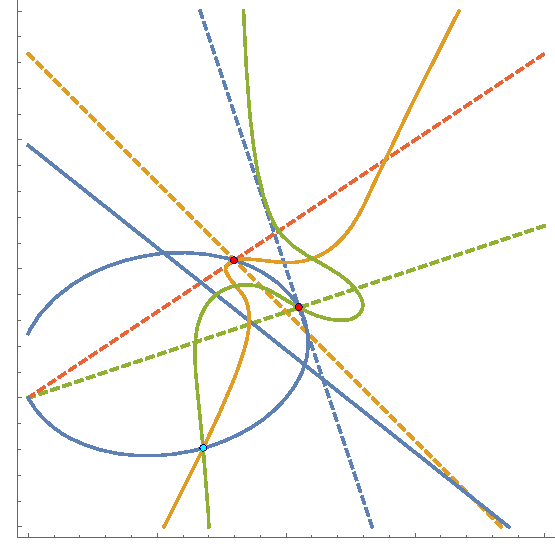
\includegraphics[width=7cm]{degree_3_example.pdf}
\end{center}

\comment{
\begin{center}
\resizebox{7cm}{!}{
\setlength{\unitlength}{266.47946777bp}%
\begin{picture}(1,1.00346963)
\put(0.0,0.0){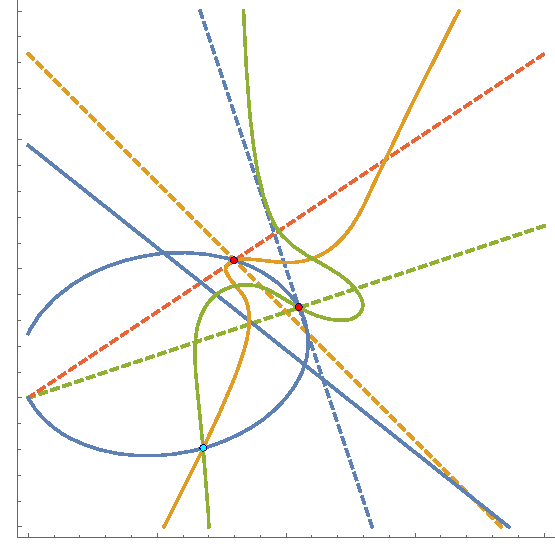
\includegraphics[width=\unitlength]{degree_3_example.pdf}}
\put(0.0348,0.0003){-2}
\put(0.27,0.0003){-1}
\put(0.5079,0.0003){0}
\put(0.7402,0.0003){1}
\put(0.9724,0.0003){2}
\put(-0.01,0.0441){-2}
\put(-0.01,0.2763){-1}
\put(0,0.5086){0}
\put(0,0.7408){1}
\put(0,0.9731){2}
\end{picture}
}
\end{center}
}

Investigating further shows us that $Z_{\bar\Q}(p_1,p_2,p_3)=Z_{\bar\Q}(q,p_2,p_3)$ and indeed, as stated in Theorem \ref{common_pts}, it consists of $m(3)=5$ points! Only one of these 5 points in 
$\P^2(\overline\Q)$ is real and this is indicated by the blue dot in the figure.
There are two red dots lying on $Z(q)$, one of them is $Z(a_{2,2},a_{2,3})$ and the other is $Z(a_{3,2},a_{3,3})$
\end{exam}

The above observation gives us an intuition for proving Theorem \ref{common_pts} especially when $d=3$

\begin{none}
Let us look more explicitly on how $b_{i,1}$ ($i>1$) is computed. In the beginning we have a system of linear equations in the 
$a_{i,1}$ for $i\ge 2$ i.e.

\begin{equation}\label{Bac_eqn}
B^\top\pmat{a_{2,1}\\ \vdots \\a_{d,1}} = \pmat{c_2 \\ \vdots \\ c_d}
\end{equation}
where $c_j$ ($j\ge 2$) are polynomials in the initial forms i.e.\ $a_{i,j}$ with either $j\ne 1$ or $(i,j)=(1,1)$. 
We obtain $b_{i,1}$
via
$$\pmat{b_{2,1}\\ \vdots \\b_{d,1}} =\adj(B^\top)\pmat{c_2 \\ \vdots \\ c_d}$$
Note that each entry of the adjugate matrix $\adj(B^\top)$ is of degree $d-2$. We then get 
\begin{equation}\label{p_and_adj}
p_i = \tilde b_{i,2} c_2 + \tilde b_{i,3} c_3 + \dots \tilde b_{i,d} c_d + q\sum_{j=2}^d a_{i,j}\alpha^{j-1} \qquad i\ge 2
\end{equation}
where $(\tilde b_{i,2} , \dots ,\tilde b_{i,d})$ is the $(i-1)$-th row of $\adj(B^\top)$.
\end{none}

%jcapco todo
\begin{none}\label{common_pts_d=3}
Let us now prove Theorem \ref{common_pts} for $d=3$. 
Since the terms with $q$ in Equation \eqref{p_and_adj} are independent of $a_{1,1}$, we can easily conclude that $Z(a_{1,1},p_2,p_3)=\emptyset$.
Thus $Z(p_1,p_2,p_3)=Z(q,p_2,p_3)$. By Bézout, $Z(q,p_i)$ for $i=2,3$ will have $6$ points. It suffices to explain how 5 out of these 6 points are the common points of the three curves 
$Z(q), Z(p_2)$ and $Z(p_3)$. 

We can explicity write   
$$\adj(B^\top) = \pmat{a_{3,3} & -a_{3,2}\\ -a_{2,3} & a_{2,2}}$$
and we are interested in the rows of this matrix.
Consider the intersection point 
$P$ of the two lines $a_{3,3}=0$ and $a_{3,2}=0$. This point is also in $Z(p_2,q)$. 
Symbolically $c_2$ and $c_3$  has terms in the initial forms that does not consist of $a_{3,3}$ and $a_{3,2}$. Therefore, by the general choice of the initial forms, the vector $(c_2, c_3)(P)$ is not 
orthogonal to $(a_{3,3},-a_{3,2})(P)$. This rules out one of the $6$ points in $Z(q,p_2)$. We claim that any point in $Q\in Z(p_2,q)$ with $Q\ne P$ is also a point
of the cubic curve $Z(p_3)$. The entries of $B$ are generic linear forms and so $q=0$ must be a smooth conic section so that the specialization $B(Q)$ is a singular 
matrix with corank 1 and the kernel of $B^\top(Q)$ is spanned by a non-trivial row of the $\adj(B^\top)(Q)$ (e.g.\ see Lemma \ref{generic_mat}\ref{coste_result}). 
In other words, $(a_{3,3},-a_{3,2})(Q)$ and 
$(-a_{2,3},a_{2,2})(Q)$ (by the general construction, this second vector is non-zero as well) differ by a non-zero scalar factor. We have therfore proven that $(c_2,c_3)(Q)$ is orthognal to both of 
these vectors and this implies that $p_2(Q)=p_3(Q)$.
\end{none}

The above proof for $d=3$ could be made easier by some cross-ratio argument. But we want to emphasize the fact that a non-trivial row of $\adj(B^\top)$ evaluated at $Q$ spans the kernel of the corank 
$1$ matrix $B^\top(Q)$. This becomes more relevant in the proof for arbitrary $d$. To prove the general case we make use of the following lemma

\begin{lemma}\label{generic_mat}
Let $A$ be a $n\times n$ matrix ($n\ge 2$) with entries being generic linear forms in $\C[x,y,z]$. We then have 
\begin{enumerate}[label=\alph*.)]
\item The zero set of $\det A$ is a smooth planar projective curve.
\item \label{coste_result} Let $P\in Z(\det A)$, the specialization $A(P)$  is a corank $1$ matrix and its kernel is spanned by a non-trivial row of $\adj(A)$.
\item \label{vanishing_row} Let $\bm v$ be a row of $\adj(A)$, then 
$$\#\{P\in \P^2(\C) \sep \bm v(P) = \bm 0\} = \frac {n(n-1)}2$$
\end{enumerate}
\end{lemma}
\begin{proof}
Smoothness is an immediate result of the fact that a determinantal 
variety is non-singular in codimension $1$ (see \cite{arbarello} \S II) and Bertini's theorem ($Z(\det A)$ is the section of a determinantal 
variety with a plane in general position). Hence, the second statement follows from \cite{coste} Lemma 2.1 and its proof.

Consider now a point $P\in \P^2(\C)$ that satsfies $\bm v(P)=\bm 0$, where $\bm v$ is the $i$-th row of 
$\adj(A)$. This means that the $(n-1)\times n$ submatrix of $A(P)$ without the $i$-th row are linearly dependent i.e. have rank $\le (n-2)$. 
Because the entries of the matrix are generic linear forms, the number 
of points at which the row $\bm v$ is zero, is the number of the points of the determinantal variety $M_{n-2}(n-1,n)$ (the points of this variety 
corresponds to $(n-1)\times n$ matrices whose corank is 
$\ge 2$) intersected with a general plane on the space of matrices. It is known that $M_{n-2}(n-1,n)$ has codimension $2$, therefore the 
intersection with a general plane is finite. This number is exactly the degree of $M_{n-2}(n-1,n)$. By the Porteous formula the degree is $\binom n2$ (see \cite{harris} Prop. 12 
or \cite{arbarello} \S II.5).
\end{proof}

\begin{proof}[Proof of Theorem \ref{common_pts}]
Similar to the proof for $d=3$ in \ref{common_pts_d=3}, we will rule out the points in $Z(q,p_2)$ for which the first row of $\adj(B^\top)$ vanishes at these points. 
By Lemma \ref{generic_mat}\ref{vanishing_row} there are $\binom {d-1}2$ such points. The rest of the proof uses exactly the same argument as the proof for $d=3$ following Lemma 
\ref{generic_mat}\ref{coste_result}. We thus have 
$$ m(d) =\# Z(q,p_2) - \binom {d-1}2 = d(d-1) - \binom {d-1}2 = \binom{d+1}2  - 1$$
\end{proof}

\section{Quintic Ternary Forms}

In this section, we will use the same notations used in Section \ref{general_sec}.
We ask whether we can follow the construction in Section \ref{general_sec} with $d=5$ to obtain a sum of 5 squares 
$\sum_{i=1}^5 p_i^2$ such that we have the finite maximum amount of real zeros for $Z(p_1,\dots, p_5)$ i.e. 
if $\# Z_{\R}(p_1,\dots, p_5) = 14$ is possible.

We will provide a strategy of obtaining such an example. 

\begin{enumerate}
\item First we choose initial forms in the $4\times 4$ matrix $B$ to be such that $\det B$ represents a curve with 
sufficiently many real inflections. Intuitively, this should provide us with a curve that is optimaly designed to 
intersect other curves at maximum number of real points. A good idea would be to choose $B$ to be the degree $4$ Taylor 
series approximation of a sinusoidal curve (because we have degree $4$, we could expand cosine at $0$ and obtain a 
degree $4$ polynomial estimate of the graph of the cosine function). Recall that that $q=\det B$.
\item Next we endow the linear forms $a_{i,1}$ for $i=1,\dots, 4$ with coefficients of $x,y,z$ that are paremetrized 
by parameters that we will want to solve. There are $15$ choices of parameters, we denote them as 
$$\bm b := b_1,\dots, b_{15}$$
\item We then obtain $p_2(\bm b;x,y,z),\dots, p_5(\bm b;x,y,z)$ paremetrized by $\bm b$
\item Furthermore, we can compute the first row of $\adj(B^\top)$ which we denote
$$\bm v := (\tilde b_{2,1},\dots, \tilde b_{5,1})$$
This is a vector of cubic forms in $x,y,z$
\item We also know the vector $\bm c$ in the right-hand side of equation \eqref{Bac_eqn} that has terms which are
quadratic in the $\bm b$.
\item We choose generic $14$ real points $P_1,\dots, P_{14} \in \P^2(\bar \Q\cap\R) \cap Z(q)$.
\item We would like to choose the parameters $b_1,\dots, b_{15}$ such that $p_2$ vanishes at $P_1,\dots, P_{14}$. 
This is the same as requiring that the inner product below vanishes
$$\spn{\bm v, \bm c}(\bm b;P_i) = 0$$
Thus we get $14$ quadratic equations in $\bm b$. 
\item Our objective is to find rational solutions (i.e.\ over $\Q$) to the $\bm b$. But this is not guaranteed. What 
is highly likely is to find a real algebraic solution $\bm b$. 
\item We then approximate $\bm b$ to rational parameters and use this. All the solutions to $Z(p,q)$ whould remain real
because $P_1,\dots, P_{14}$ was initially chosen generically (thus they should not be points were $\bm v$ vanishes) 
and real and so the new rational approximate to $\bm b$ will give us a slight perturbation of $P_1,\dots,P_{14}$ as 
points of $Z(p,q)$ which remain real.
\end{enumerate}

\section{conjecture}

Let $K:= \Q(\alpha)$ for some algebraic number $\alpha$ of degree $d=[K:\Q]>1$. 
Consider an element $P\in\P^n(K)$, then we say that $P$ is $\Q$-rational if there is a representative
$P=(p_0:p_1:\dots:p_n)$ with $p_i \in \Q$. We say that $P$ is a {\it general point over $K$} if for a 
representative $(p_0:p_1:\dots :p_n)$ of $P$, the coordinates $p_i$ generate a $\min(d,n)$-dimensional $\Q$ vector 
subspace of $K$ (thus all representatives of $P$ generate such a subspace). Similarly we define a {\it general 
hyperplane over $K$} by identifying points in $(\P^n)^*$ with points in $\P^n$. Thus, if $\beta$ is an algebraic 
number of degree $d>n$. Then immediately from the definition, a general hyperplane in $\P(\Q(\beta))^n$ will have no 
$\Q$-rational point. More generally we have the following Lemma

\begin{lemma}\label{l-qrational}
If $\beta$ is an algebraic number of degree $d$, then a general linear space of 
dimension less than $d-1$ in a projective space $\P^n(\Q(\beta))$ with $n\ge d-1$ has no $\Q$-rational point.
\end{lemma}

Now consider our construction of $d$-adic ternary forms. By a {\it general construction with maximum number of real 
points} we mean one such that 
\begin{itemize}
\item $Z(p_1,\dots, p_d)$ has maximum number of real points i.e. $M:=\binom{d+1}2-1$ different real points which we 
denote $P_1,\dots, P_M$.
\item The points $P_i$ are general over $K:=\Q(\beta)$ where $\beta$ is a real algebraic number of degree $M$.
\item The points $P_i$ are in sufficiently general position in $\P^2(K)$ (this will be made precise).
\end{itemize}

We want to prove the following claims 
\begin{itemize}
\item For any $d\ge 3$ such a construction is possible 
\item For such a construction, the sum of squares of these $d$-adic ternary forms is not $\Q$-sos.
\end{itemize}

\begin{none}
We start with the moduli space of planar curves of degree $d$, this is the projective space of dimension 
$$N := \binom{d+2}2 -1 $$
%see Beltrammeti \S p172, p'188, Remark 6.3.2
This is also a regular linear system, so that we can choose real points $P_1,\dots, P_M$ defined over $\Q$ (i.e.\ the 
set of these points is the zero set of a system of polynomial equations over $\Q$) general enough such that: 
$P_i$ is a $\Q(\beta)$-rational for some real algebraic number $\beta$ of degree $M$ and general over $\Q(\beta)$;
each $P_i$ imposes an independent linear condition to the linear system (the third condition above). So that with the 
base points $P_1,\dots, P_M$, we have a 
new linear system of dimension $N-M=d+1$. By Lemma \ref{l-qrational}, there are 
no non-trivial form over $\Q$ of degree $d$ that has all these $P_i$ as zero.
\end{none}

%jcapco now
From the above argument, we see that we can relax the condition for $M$. We need not require $M$ to be the 
maximum number of real points. It suffices to satisfy the two last 
conditions and instead of $M=\binom{d+1}2-1$ for the first condition, we simply require that $M > N-M$ i.e. 
% M>N-M \ge d+1
\begin{prop}
A general construction of $2d$-adic ternary form over $\Q$ ($d\in 2\N+1$) such that 
\begin{itemize}
\item $Z(p_1,\dots, p_d)$ has at least $M$ real points with 
$$ M > \frac{d(d+3)}4$$
\item The points $P_i$ are general over $K:=\Q(\beta)$ where $\beta$ is a real algebraic number of degree $M$.
\item The points $P_i$ are in sufficiently general position in $\P^2(K)$.
\end{itemize}
is not $\Q$-sos.
\end{prop}

\noindent
Thus, we see that for $d=3$ we need $M$ to be the maximum number of real points ($5$ points) and for $d=5$ it 
suffices to have $14\ge M \ge 11$ real points. %($M=14$ is the maxumum number of real points for $d=5$).


\bibliographystyle{amsplain}
\bibliography{rationalSOS}

\end{document}
